\chapter{Implementierung der Client-Applikation}
\label{cha:impl_device}

\section{Technologische Grundlagen}
\subsection{Android}
Wie bei der Vorstellung der verwendeten Smartglass Vuzix M100 bereits erwähnt wurde, setzt die Datenbrille auf dem Betriebssystem Android auf. Android ist eine Open-Source-Plattform für Mobilgeräte, welche durch Google bekannt geworden ist und der Open Handset Alliance gehört. Es soll ein Mittel für eine beschleunigtere Innovation im Mobilbereich sein, welches dem Anwender ein besseres Mobilerlebnis bieten soll, und ist seit 2008 auf dem Markt.\footnote{\citep{android_general}}\\
Android ist eine Plattform, die es ermöglicht, Anwendungen unabhängig von der ausführenden Hardware zu schreiben. Dazu setzt Android auf Java, welches um ein eigenes Android SDK erweitert wird, mit dem die speziellen Funktionen der Mobilgeräte angesprochen werden können. Anwendungen (Apps) werden als Pakete (APK-Dateien) auf einem Android-Gerät installiert. Eine solche App wird für \acs{SMAR} entwickelt und auf der Smartglass installiert.

\subsection{Multithreading}
Komplexe Anwendungen, die Anfragen oder Funktionen beinhalten, welche mehrere Sekunden bis zu Minuten für die Bearbeitung der Anfrage benötigen, müssen in mehrere Threads aufgeteilt werden, um dem Benutzer zu vermitteln, dass die Anwendung nicht abgestürzt ist. Anwendungen mit vielen Netzwerkanfragen, wie \zB \ac{SMAR}, sind ein gutes Beispiel dafür.\\

Anwendungen, die nur einen Thread benutzen, werden ausschließlich sequentiell ausgeführt. Wird eine Anfrage ausgeführt, die mehrere Sekunden benötigt, blockiert die Anfrage den Prozessor und die Anwendung. Die Anwendung kann sich daher nicht mehr aktualisieren -- dies betrifft ebenfalls das \ac{UI}. Ein Ladebalken würde daher ebenfalls stehen bleiben, sodass der Benutzer nicht über einen Fortschritt informiert werden kann und nach wenigen Sekunden denken wird, dass die Anwendung nicht mehr reagiert und abgestürzt ist. Dazu kommt, dass das Android System die Anwendungen kontrolliert und feststellt, dass eine Anwendung nicht reagiert. Nach ca. fünf Sekunden bekommt der Benutzer vom Android System einen Dialog angezeigt: \glqq Aktivität [NAME] reagiert nicht.\grqq\ und den Auswahlmöglichkeiten \glqq Schließen erzwingen\grqq\ und \glqq Warten\grqq . Dies unterstreicht die Meinung des Benutzers, dass die Anwendung abgestürzt ist. Eine gute Usability, welche aussagt, dass ein System zu jeder Zeit reagieren sollte, ist nicht mehr gegeben.\\

Das folgende Beispiel soll verdeutlichen, wann solch ein Fall eintreten kann: Die \ac{SMAR}-App schickt eine Anfrage an den \ac{SMAR}-Server, der angenommene Ware einspeichern soll. Da das Firmennetzwerk gerade überlastet ist, wird die Anfrage erst nach einigen Sekunden bearbeitet. Der Benutzer empfängt, statt eines bewegten Ladebildschirms, den Dialog des Android Systems und schließt die Anwendung. Jegliche Arbeitsfortschritte gehen verloren. Dies wäre für einen Einsatz in großen Filialen fatal, da ein inkonsistenter Warenbestand die Folge wäre.\\

Die gängige Lösung ist das Aufteilen der Anwendung auf mehrere Threads, wobei jedem Thread eine bestimmte Aufgabe zugeordnet wird. Eine sinnvolle Aufteilung in \ac{SMAR} sieht folgendermaßen aus:
\begin{itemize}
	\item Main-Thread: Verwaltung aller weiteren Threads
	\item UI-Thread: Anzeige der Oberfläche (mit Informationen, die in anderen Threads generiert werden), sowie Weiterleitung von Benutzerinteraktionen
	\item Scanner-Thread: Zuständig für das Scannen der Barcodes
	\item Netzwerkkommunikation-Thread: Sendet Netzwerkanfragen an den Server und liefert die Ergebnisse zurück
\end{itemize}
Diese Threads können über Java durch die Erweiterung der Klasse \textit{java.lang.Thread} einfach erstellt und verwendet werden.\footnote{\citep[S. 18ff.]{java_threads}}\\

Die Architektur von Android empfiehlt diese Vorgehensweise jedoch nicht. Das Android System erstellt einen Thread für jede gestartete App, auf welchem die Anwendung sequentiell abläuft. Dieser Thread wird von Google auch \ac{UI}-Thread genannt, da dieser der einzige Thread ist, welcher mit dem \ac{UI} interagiert und interagieren darf. Andere Threads sollen das \ac{UI} nicht bearbeiten, was die oben vorgestellte Architektur verletzt, da diese Threads die Informationen in dem \ac{UI} eintragen müssen oder mit dem \ac{UI}-Thread synchronisiert werden müssen. Diese Synchronisierung ist sehr kompliziert und würde den Rahmen dieser Arbeit sprengen.\\

Android bietet stattdessen \glqq ASyncTasks\grqq , also eine Klasse für Asynchrone Aufgaben, an. Diese Klasse muss durch \ac{SMAR}-eigene Klassen erweitert werden, die in die bereitgestellten Methoden die durchzuführenden Aufgaben implementieren. Diese asynchrone Aufgabe wird dabei durch einen neuen Thread im Hintergrund ausgeführt, während der UI-Thread  annähernd\footnote{Annähernd, da der Prozessor nur eine Aufgabe gleichzeitig ausführen kann, aber die Threads abwechselnd für eine kurze Dauer ausführt, sodass dies für den Benutzer parallel wirkt.} parallel im Vordergrund weiter ausgeführt wird und somit die Ausgabe (wie \zB einen bewegten Ladebildschirm) ständig aktualisiert.\\
Sobald die asynchrone Aufgabe vollständig ausgeführt wurde, wird das Ergebnis an eine Methode der ASyncTasks-Klasse übergeben, die auf dem UI-Thread ausgeführt wird. Dadurch wird  die Ausgabe auf dem UI-Thread verändert und die von Google vorgesehene Architektur wird nicht verletzt.\footnote{\citep[S. 115ff.]{android_threads}}

\subsection{Barcode-Erkennung}
\label{sec:barcode}
Dieses Kapitel beschäftigt sich mit der Implementation der Barcode Scanner-Funk\-tion in die \ac{SMAR}-Anwendung auf der Smartglass. Wie im Kapitel \ref{cha:technik} \nameref{cha:technik} bereits beschrieben, fiel die Entscheidung gegen die Anschaffung eines externen Barcode-Scanners, sodass die Erkennung von Bar- und QR-Codes durch eine Library in Verbindung mit der eingebauten Kamera übernommen wird.\\

Android \bzw Google bieten keine Library für das Erkennen von Bar-/QR-Codes an. Außerdem würde es den Rahmen dieses Projektes übersteigen, eigene Klassen für diese Aufgabe zu entwickeln. Eine Recherche ergab folgende zwei populäre und ausgereifte, externe Librarys, die frei zur Verfügung stehen:
\begin{itemize}
	\item zebra crossing (ZXing)
	\item ZBar SDK
\end{itemize}
Bei ZXing handelt es sich in erster Linie um eine Barcode-Scanner-App für Android. Darüber hinaus unterstützt die App jedoch den externen Zugriff durch eine andere App und kann das Ergebnis des Scans an die externe App weitergeben. Das \ac{SMAR}-Projekt würde die Barcode-Scanner-App von ZXing entsprechend jedes mal starten, sobald ein neuer Code benötigt wird und die Antwort der Barcode-Scanner-App abwarten.\\
Ein großer Vorteil ist die schnelle und einfache Integration, die anhand weniger Zeilen Sourcecode geschieht. Entscheidende Nachteile sind jedoch die Abhängigkeit von einer anderen App, die auf dem Gerät ebenfalls installiert sein muss, und der erhöhte Ressourcenverbrauch, der die \ac{SMAR}-App in der Effizienz einschränken könnte. Da der Sourcecode der Barcode-Scanne- App frei verfügbar ist, gäbe es die Möglichkeit, die gesamte Anwendung zu integrieren. Dies ist aufgrund der Komplexität aber ebenfalls nicht praktikabel.\\

Die Entscheidung fiel daher auf die ZBar SDK Library. Diese wird in das Projekt als externe Library integriert und bietet die Möglichkeit, Bilder auf einen Bar- oder QR-Code zu untersuchen. Ein Nachteil ist der erhöhte Programmieraufwand, der für das Erstellen der Kameravorschau und der Aufruflogik benötigt wird. Der entscheidende Vorteil ist jedoch, dass alle Aktionen innerhalb der \ac{SMAR}-Anwendung stattfinden und keine externen Anwendungen zur Laufzeit benötigt werden.\\

Die ZBar Library unterstützt alle gängigen Barcode- und QR-Code-Typen und ist damit optimal für den Einsatz in diesem Projekt geeignet:\footnote{\citep{zbar}}
\begin{itemize}
	\item EAN/UPC: EAN-8, EAN-13, UPC-A, UPC-E
	\item Linear: Code 39, Code 93, Code 128, Interleaved 2 of 5, DataBar
	\item 2-D: QR-Code
\end{itemize}

Für die Integration der ZBar Library werden zwei neue Klassen benötigt:
\begin{enumerate}
	\item Eine Activity (eine neue Ansicht in der App), im folgenden Barcode-Klasse genannt.
	\item Eine Klasse, welche die Kameravorschau innerhalb eines Fensters erstellt, das in eine Activity eingebunden werden kann; im folgenden Kamera-Klasse genannt.
\end{enumerate} 
Soll ein Barcode eingescannt werden, so wird die Barcode-Klasse aufgerufen. Diese erstellt eine neue Instanz der ZBar Library mit entsprechend eingestellter Konfiguration (wie \zB Auflösungseinstellungen oder zu erkennende Codes) und fragt beim Android-Betriebssystem nach der Öffnung einer Kamerainstanz. Wird eine gültige Kamerainstanz zurückgeliefert, so wird die Kamera-Klasse mit dieser Instanz ausgeführt und das Vorschaubild in die Activity integriert. Außerdem stellt die Barcode-Klasse Methoden zur Verfügung, die bei Rückgabe von Werten seitens der Kamera-Klasse ausgeführt werden. Dies sind die Bilder, die die Kamera aufzeichnet, die anschließend an die Instanz der ZBar Library weitergeleitet werden. Liefert die ZBar Library ein Ergebnis zurück, so wird die Kamera-Klasse, die Kamerainstanz sowie die Activity geschlossen und die Barcode-Klasse gibt das Ergebnis zurück. Dieses Ergebnis kann mit der Klasse, die die Barcode-Klasse ausgeführt hat, über eine Methode (\emph{onActivityResult}) abgerufen werden.\\

Die Kamera-Klasse konfiguriert bei Ausführung zunächst die Kamera (Ausrichtung der Kamera, Bildwiederholrate, Autofokus, ...) und definiert den Callback. Der Callback wird ausgeführt, sobald die Kamera ein Bild aufgenommen hat. Als Daten werden dabei die Bildinformationen übergeben, die von der Barcode-Klasse abgerufen werden.

\subsection{Visualisierung der Regale}
Für einige Prozesse auf der Datenbrille ist es erforderlich, dass die exakte Position eines Produktes in einem Regal auf der Verkaufsfläche angezeigt wird. Dazu gibt es unter Verwendung von Wearable-Computern grundsätzlich zwei Möglichkeiten:

\begin{enumerate}
	\item Das Regal wird abstrahiert und schematisch in einer vereinfachten Form dargestellt. Innerhalb dieser Darstellung wird die Position des gesuchten Produktes im Regal markiert. Der Benutzer muss selbst die Verknüpfung zwischen der Darstellung und der Realität herstellen, wenn er vor dem Regal steht.
	\item Durch Nutzung einer Videokamera wird die Umgebung des Benutzers und somit das Regal digital erfasst und durch Bild-im-Bild-Überlagerung die Produktposition im Regal markiert. Die Verknüpfung von Darstellung und Realität ist dadurch sehr stark. Voraussetzung ist hierbei jedoch, dass der Benutzer sich direkt vor dem Regal befindet -- andernfalls ist wiederum eine abstrahierte Darstellung erforderlich.
\end{enumerate}

Für die Umsetzung des Systems im Rahmen dieser Arbeit wurde die erste Möglichkeit gewählt, da sie technisch einfacher umzusetzen ist und zugleich auch eine Umsetzung der zweiten Möglichkeit vorbereitet.

Für die schematische Darstellung des Regals wurde die Ansicht gewählt, die ein Benutzer hat, wenn er sich vor dem Regal befindet (Frontalansicht oder Draufsicht). Regale sind rechteckig, ebenso wie Regalfächer, und lassen sich jeweils über Höhe und Breite, sowie bei den Fächern über die Position im Regal beschreiben. Dies sind optimale Voraussetzungen für die Umsetzung als zweidimensionale Ansicht.

Die technische Umsetzung der schematischen Darstellung kann i.A. auf drei Arten erfolgen:

\begin{enumerate}
	\item als Bitmap (pixelbasierte Grafik);
	\item als Vektorgrafik, also eine mathematisch beschriebene Grafik, die bei Ausgabe auf Bildschirmen verlustfrei in eine Bitmap der gewünschten Auflösung umgewandelt wird; 
	\item als \acs{3D}-Grafik, die zusätzlich noch Tiefeninformationen speichert.
\end{enumerate}

Für die Darstellung auf dem Gerät fiel die Entscheidung auf eine Umsetzung als Vektorgrafik im \acs{SVG}-Format. Eine \acs{SVG}-Grafik ist im Grunde eine \acs{XML}-Datei, besteht also aus Text. Grundformen wie Rechtecke lassen sich über \acs{SVG} sehr einfach beschreiben, und für die Darstellung eines Regals werden keine komplizierteren Formen benötigt. Dies ist sehr speicherplatzsparend im Vergleich zu Bitmaps mit demselben visuellen Inhalt. Außerdem können im \acs{XML}-Code der \acs{SVG}-Grafik weitere Informationen über das Regal und die Fächer hinterlegt werden, wie z.B. die entsprechenden IDs der Fächer und Produkte aus der Datenbank. Nicht zuletzt ist die verlustfreie Skalierbarkeit der Vektorgrafik ein unschätzbarer Vorteil, der das Grafikformat unabhängig von der Größe der Ausgabe macht und somit die Geräteunabhängigkeit der Applikation wesentlich verbessert.

Für SMAR sind daher alle Regale als \acs{SVG}-Grafiken angelegt. Die Grafiken werden bei Anlegen eines Regals in der Webadministration automatisiert erzeugt und in einer eigenen Tabelle (\textbf{\textit{shelf\_graphic}}) gespeichert. Bei Updates für ein entsprechendes Regal (z.B. Bearbeiten des Regals oder von darin enthaltenen Fächern) wird die \acs{SVG}-Grafik neu generiert und in der Tabelle aktualisiert. Die Grafik selbst enthält neben der Darstellung auch die IDs der Fächer, um diese später einfach erst referenzieren und dann ansprechen zu können.

Die Smartglass selbst lädt bei Start der App automatisch den neuesten Stand der \acs{SVG}-Grafiken aus der Datenbank herunter und speichert die Grafiken lokal als Dateien ab. Wird eine Regal-Darstellung benötigt, kann diese direkt aus dem lokalen Speicher der Smartglass geladen werden. Dies spart während der Nutzung der Brille Traffic und erhöht somit die Performance der Anwendung. Soll außerdem ein Regalfach markiert werden, kann direkt der \acs{XML}-Code der \acs{SVG}-Grafik manipuliert werden -- z.B. kann über die angeheftete ID eines Faches die entsprechende Rechteck-Form gesucht und über entsprechende \acs{SVG}-Anweisungen eingefärbt werden.


\section{Interaktionsprozesse}

\subsection{Produkt finden}
\label{sec:produkt_finden}
Dieser Abschnitt beschreibt, wie ein Mitarbeiter mithilfe der Smartglass einen Produktplatz finden kann. Dies wird anhand eines Sequenzdiagramms veranschaulicht. Die Voraussetzung für diesen Prozess ist, dass der Anwender den Menüpunkt \glqq Produkt finden\grqq  im Hauptmenü ausgewählt hat.

Wie die folgende Grafik zeigt, gibt es drei Akteure, die miteinander kommunizieren: den Mitarbeiter, die Smartglass und die Datenbank (REST API).
\begin{figure}[H]
	\centering
	{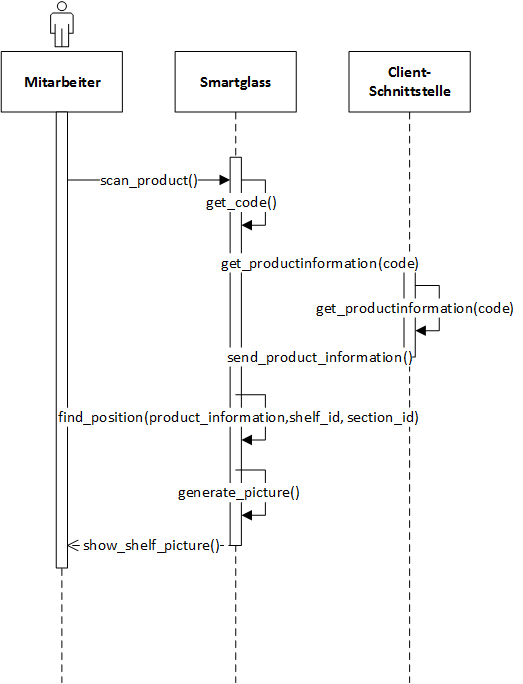
\includegraphics[scale=0.8]{Bilder/Abbildungen/SMAR_produkt_finden_Sequenzdiagramm.png}}
	\caption{Sequenzdiagramm: Produkt finden}
	\label{fig:sequenz_finden}
\end{figure}
Nachdem der Mitarbeiter die Funktion gestartet hat, vermittelt er der Smartglass den Befehl ein Produkt zu finden, sodass die Smartglass sofort in den Scan-Modus springt (\emph{scan\_product()}). 

Sofern der Artikel gescannt wurde, berechnet die Smartglass aus dem Bild den entsprechenden Barcode (\emph{get\_code()}). Dies geschieht mit der ZBar Library. Nachdem die Smartglass den Barcode errechnet hat, verschickt sie diesen Code an die Client-Schnittstelle auf dem Server, der sich im gleichen Netzwerk befindet. Mithilfe des Barcodes sucht die Datenbank intern nach dem entsprechenden Produkt. Anschließend werden über das Produkt folgende Informationen zurück an die Smartglass geschickt:
\begin{itemize}
	\item Der Name zur ergonomischen und leichten Handhabung für den Mitarbeiter.
	\item Die Füllstände von dem Artikel auf der Verkaufsfläche und im  Lager.
	\item Die aktuell ausgewählte Unit (Karton, Einzelstück).
	\item Die zugehörige Shelf-ID als auch die entsprechende Section-ID zur Positionsangabe.
\end{itemize}
Der Name sowie die Füllstände im Lager und im Verkauf werden dem Nutzer angezeigt.

Mithilfe der Produktinformation und den hinterlegten \acs{SVG}-Grafiken aller Produktplätze generiert die Smartglass ein Bild (\emph{generate\_picture()}). Die \acs{SVG}-Grafik enthält im \acs{XML}-Code Informationen zu den enthaltenen Regalplätzen. Mithilfe der Positionsinformationen aus der Datenbank kann die Smartglass die passende Grafik laden und den Regalplatz entsprechend markieren, in den das Produkt einzuräumen ist. Dieses Bild wird dem Mitarbeiter anschließend angezeigt. (\emph{send\_shelf\_picture()}).

Da in den meisten Fällen nach der Produktplatzsuche das jeweilige Produkt eingeräumt werden soll, fragt die App den Mitarbeiter, ob er in den Einräummodus wechseln möchte.
Bestätigt er, springt der \textit{Instruction Pointer} in den Prozess \glqq Produkt einräumen\grqq ; dort wird allerdings der Scan-Vorgang übersprungen und direkt der Dialog mit den bereits bekannten Produktinformationen geöffnet. Verneint der Nutzer, so springt die Smartglass zurück an den Anfang des \glqq Produkt finden\grqq -Prozesses. \\
Wie das Ergebnis letztlich aussieht zeigt folgendes Mockup. Hierbei ist zu beachten, dass dies nicht 100\% der tatsächlichen Umsetzung entspricht. 
\begin{figure}[H]
	\centering
	{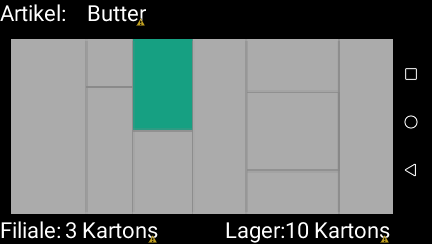
\includegraphics[scale=0.7]{Bilder/Abbildungen/produkt_finden_mockup.png}}
	\caption{Mockup: Produkt finden}
	\label{fig:jwt_encode}
\end{figure}

\subsection{Produkt einräumen}
Dieser Abschnitt gibt Implementierungsdetails sowie architektonische Einblicke in die Umsetzung des Prozesses \glqq Produkt einräumen\grqq . Dabei soll die Umsetzung anhand des folgenden Sequenzdiagramms chronologisch beschrieben werden. Vorausgesetzt ist, dass der Mitarbeiter schon die Funktion \glqq Produkt einräumen\grqq~ ausgewählt hat. 

\begin{figure}[H]
	\centering
	{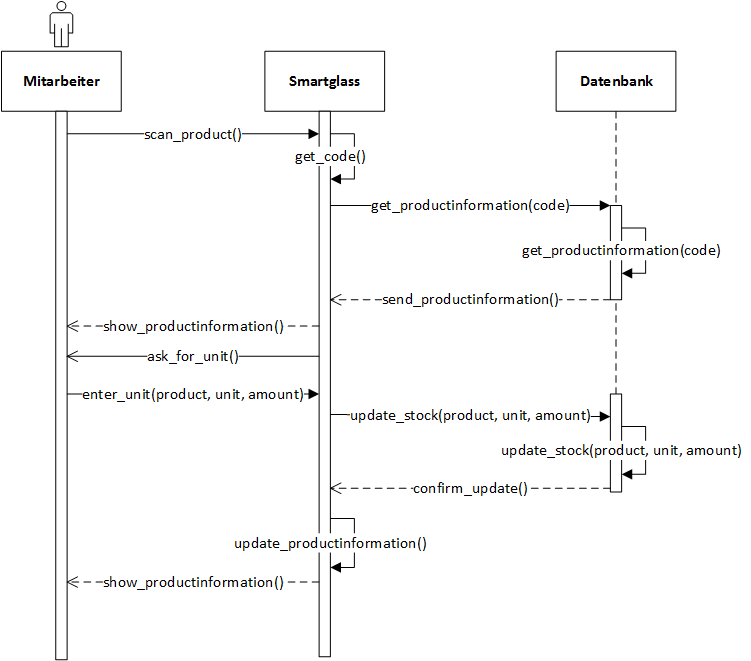
\includegraphics[scale=0.7]{Bilder/Abbildungen/SMAR_produkt_einraeumen_Sequenzdiagramm.png}}
	\caption{Sequenzdiagramm: Produkt einräumen}
	\label{fig:sequenz_einraeumen}
\end{figure}

Ähnlich dem Prozess \glqq Produkt finden\grqq~ gibt es drei Akteure: den Mitarbeiter, die Smartglass und die Datenbank (REST API). Zunächst öffnet die Smartglass den Barcodescanner und ermittelt den sichtbaren Barcode (\emph{get\_code()}). Dieser Code wird mit der Aufforderung, produktspezifische Informationen zurück zu geben,  an die REST API verschickt (\emph{get\_productinformation()}). Die Client-Schnittstelle fragt diese Informationen von der Datenbank ab und antwortet der Smartglass mit den Produktdaten (\emph{send\_productinformation()}). Bei diesen Informationen handelt es sich um folgende: 
\begin{enumerate}
	\item Der Name zur ergonomischen und leichten Handhabung für den Mitarbeiter.
	\item Die Füllstände von dem Artikel auf der Verkaufsfläche und im  Lager.
	\item Die aktuell gescannte Unit (Karton, Einzelstück).
\end{enumerate}
Die gescannte Unit ist dabei der Barcode an einem Karton oder einem einzelnen Produkt. So kann die einzuräumende Unit (und damit auch die Menge) vorselektiert werden. Diese Informationen werden dem Mitarbeiter auf dem Display angezeigt. Dies ist auch der Punkt, an dem der Prozess \glqq Produkt finden\grqq~ in diesen Prozess springt, sollte der Mitarbeiter von dort aus in den Einräummodus wechseln -- so muss der Mitarbeiter weniger mit der Smartglass interagieren, sodass Zeit gespart wird. Er hat allerdings noch die Möglichkeit, die Unit entsprechend anzupassen (\emph{ask\_for\_unit()} und \emph{\emph{enter\_unit()}}). Dabei kann nicht nur die Unit angegeben werden (ob Karton oder Einzelstück), sondern auch die Anzahl (\zB 4 Kartons); damit soll die mehrfache Interaktion vermieden werden. 

Schließlich bestätigt der Mitarbeiter (\emph{enter\_unit()}) und die Smartglass leitet die neuen Informationen an die API weiter (\emph{update\_stock()}). So werden dort die Füllstände für das Lager und auf der Verkaufsfläche entsprechend angepasst (\emph{update\_stock()}).

Die Datenbank bestätigt dies (\emph{confirm\_update()}), die Smartglass aktualisiert die Informationen, die dem Nutzer angezeigt werden (insbesondere die Füllstände) (\emph{show\_productinformation()}), und springt schließlich zurück zum Anfang des Prozesses. 


\subsection{Warenannahme}
Dieser Abschnitt beschreibt den Interaktionsprozess zwischen dem Mitarbeiter, der Smartglass und der Datenbank (REST API) während der Warenannahme. Wie in den vorherigen Abschnitten wird ein Sequenzdiagramm zur Veranschaulichung verwendet. Voraussetzung für diesen Prozess ist, dass der Mitarbeiter den Prozess \textit{Warenannahme} im Hauptmenü ausgewählt hat.\\

Ist dies geschehen, öffnet die Smartglass den Scanmodus und erwartet vom Mitarbeiter, dass dieser den Code auf dem Bestellschein einscannt. Der Bestellschein ist deshalb wichtig, damit die Waren, die im Folgenden erfasst werden, der entsprechenden Bestellung zugeordnet werden können (\emph{scan\_delivery\_note()}).\\
Wurde der Code eingescannt, so wird anhand des ermittelten Codes über die Client-Schnittstelle die Positionsliste der Bestellung angefragt (\emph{get\_delivery\_information()}). Die API ermittelt die erwartenden Produkte und Mengen (\emph{get\_delivery\_information()}) und sendet diese als Liste zurück an die Smartglass (\emph{send\_information()}), welche diese dem Mitarbeiter anzeigt (\emph{show\_delivery\_information()}).\\

Wie in der Schleife zu sehen, wiederholt sich der nun folgende Vorgang solange, bis entweder der Bestellschein abgearbeitet ist oder der Mitarbeiter diesen Vorgang unterbricht. Der Mitarbeiter scannt einen Artikel \bzw Karton der Lieferung (\emph{scan\_product()}). Daraufhin ermittelt die Smartglass den Code, verschickt diesen an die Client-Schnittstelle, sodass diese mit entsprechenden Produktinformationen antworten kann. So ist eine Zuordnung zwischen dem gescannten Produkt und der folgenden Auswahl von einzuräumender Kartongröße und deren Anzahl möglich. Hat der Mitarbeiter diese Daten eingetragen und bestätigt, so werden diese in einer Liste auf der Smartglass gespeichert.\\

Ist der Mitarbeiter fertig, wird ihm eine Differenzliste angezeigt. Diese setzt sich aus den bestellten und den gelieferten Mengen zusammen. So hat der Mitarbeiter den Überblick und kann im nächsten Schritt den Vorgang abschließen.\\
Bei Abschluss der Warenannahme werden die Lagerbestände der Produkte entsprechend der Eingaben des Nutzers im Lager erhöht. Außerdem werden neue Einträge in der Datenbank angelegt, welche die Lieferung abbilden, um später z.B: eine Differenzliste über die Webadministration zu erstellen. Damit der Mitarbeiter eine Rückmeldung am Ende seiner Arbeit bekommt, erscheint eine kurze Erfolgsmeldung (\emph{success\_delivery\_scan()}).

\begin{figure}[H]
	\centering
	{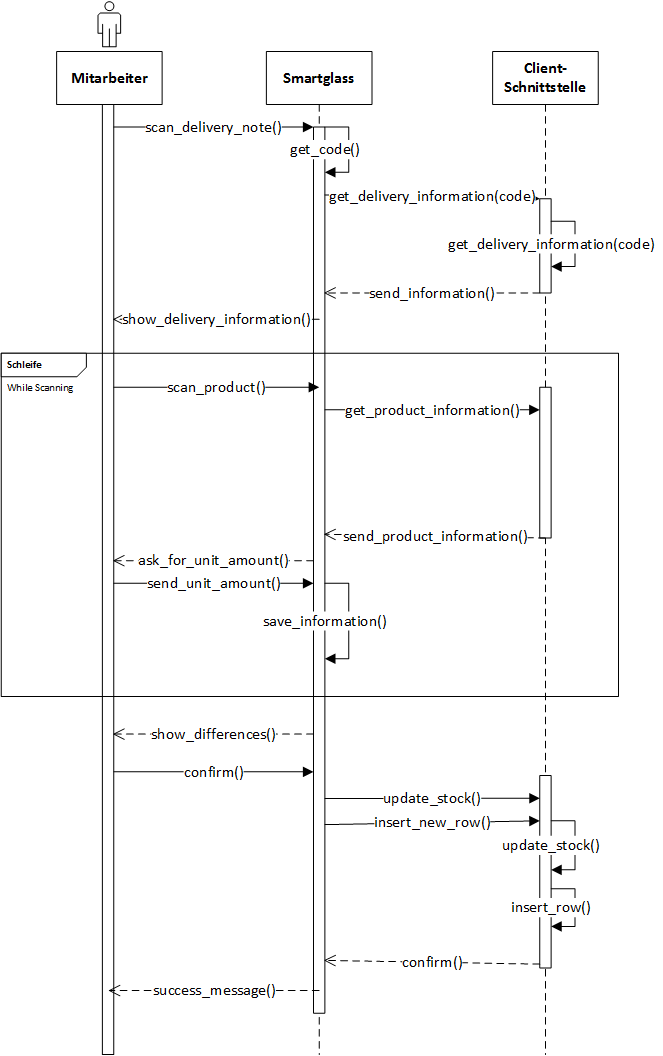
\includegraphics[scale=0.75]{Bilder/Abbildungen/SMAR_warenannahme_Sequenzdiagramm.png}}
	\caption{Sequenzdiagramm: Warenannahme}
	\label{fig:sequenz_warenannnahme}
\end{figure}

\section{HTTP Nutzung}
\label{sec:httpnutzung}
Dieser Abschnitt befasst sich nicht mit einem konkreten Prozess, sondern erklärt das allgemeine Vorgehen und die Akteure bei einem der vielen REST API Aufrufe. Voraussetzung für eine einwandfreie Nutzung der REST API sind zwei Pakete auf der Smartglass. Diese sind standardmäßig ausgeliefert und müssen somit nicht manuell nachinstalliert werden:
\begin{enumerate}
	\item org.apache.http
	\item org.json.JSONObject
\end{enumerate}
Das erste Paket enthält die Hauptklassen und -methoden zur Nutzung von HTTP Komponenten. Diese sind essentiell, um das HTTP-Protokoll zu verwenden; darüber können zum Beispiel HTTP-Verbindungen geöffnet, Requests versendet und Responses entgegen genommen werden.\footnote{\citep{http}} Mit Hilfe des zweiten Pakets können JSON-Objekte erstellt und bearbeitet werden. \footnote{\citep{json}}\\

Das folgende Klassendiagramm visualisiert die nötigen Klassen, um einen HTTP-Request zu versenden, eine Antwort zu erhalten und schließlich die Daten daraus zu verwenden.

\begin{figure}[H]
	\centering
	{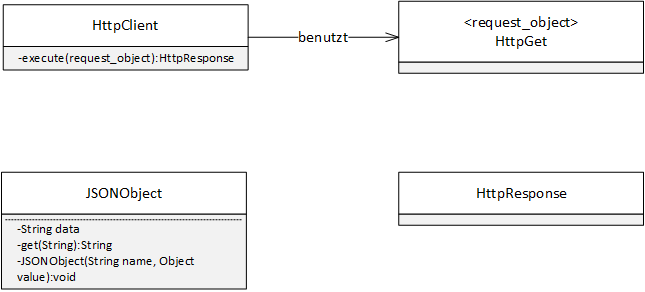
\includegraphics[scale=0.7]{Bilder/Abbildungen/http_request_klassendiagramm.png}}
	\caption{Klassen zur Verwendung von HTTP-Requests}
	\label{fig:http_klassen}
\end{figure}

Zu Beginn wird ein Objekt der Klasse \emph{HttpClient} erzeugt. Der HttpClient kann ein sogenanntes \emph{request\_object} erzeugen -- konkret in der Grafik ein \emph{HttpGet}-Objekt. Grundsätzlich sind aber auch HttpPost, HttpDelete und HttpPut, nur um die wichtigsten HTTP Verben zu nennen, möglich. Der Instanz der Klasse HttpGet wird eine URL zugewiesen, und anschließend benutzt das Objekt HttpClient, mithilfe der \emph{execute}-Methode, das \emph{request\_object}.\\

Wird dieser Befehl ausgeführt, so wird ein Http-Request an den Server geschickt. Dieser antwortet mit einem einfachen HttpResponse, bestehend aus Header und Body. Sofern der Request korrekt und ohne Fehler durchlaufen ist, ist der Body des Response nicht leer. Somit kann er mithilfe eines Objekts der Klasse HttpResponse angenommen werden. Die Daten können nun als String weiterverarbeitet werden.\\

Die HttpResponses sind in diesem konkreten Projekt in \acs{JSON}-Syntax geschrieben, sodass die Antworten des Servers leicht verwendet werden können. Dies ist mithilfe eines JSON-Objektes simpel zu realisieren. Dazu wird die Methode bzw. auch der Konstruktor mit dem entsprechendem String gefüllt. Die Umwandlung des Strings in einzelne Attribute übernimmt das Objekt selbst. Mithilfe der Methode \textit{get(String)} können einzelne Attribute herausgezogen werden, indem als \textit{String} der Name des Attributes angegeben wird.\\

Somit lassen sich die vielen HTTP-Aufrufe, also die Interaktion mit den REST-Services der Client-API, sehr einfach nutzen und verarbeiten.

\section{Settings}
\label{sec:settings}
Prinzipiell werden in einer Applikation unter einer Android-Umgebung Informationen in einem sogenannten SharedPreferences-Pool gespeichert. Diese sind in der ganzen Applikation verfügbar und enthalten die gespeicherten Einstellungen als Key-Value-Pairs (Schlüssel-Wert-Paare). Dazu wird der Pool der aktuellen Applikation geladen und über einen Editor editierbar gemacht. So können Einstellungen verändert werden.\\
Ähnlich verläuft das Abrufen von Einstellungen. Dazu werden ebenfalls über die aktuelle Applikation die \emph{SharedPreferences} aufgerufen und darin der Name der Einstellung herausgesucht. Anschließend erhält man den Wert der Einstellung.\\

Die Speicherung von Einstellungen auf der Smartglass wird mit der Klasse \emph{PreferencesHelper.java} organisiert, welche Hilfsfunktionen zur einfacheren Speicherung von Einstellungen enthält. Damit wird eine Abstraktionsschicht für jegliche Zugriffe auf Einstellungen bereitgestellt. So laufen alle Zugriffe gleich ab, und bei Änderungen oder Erweiterungen braucht nur die Helper-Klasse bearbeitet werden. Dennoch sind alle nutzenden Klassen von Veränderungen betroffen. 


\section{Rechteverwaltung}
\label{cha:rechteverwaltung_vr}

\subsection{\acf{AuthN}}
Das folgende Kapitel beschäftigt sich mit der Authentifizierung in der App gegenüber dem Server. Benutzte Bibliotheken und Eingabemethoden werden erklärt und die verwendete Methode mit anderen technisch möglichen Eingabemethoden verglichen.

\subsubsection{\acs{AuthN} gegenüber der Brille}
Die App auf der eingesetzten Vuzix M100 Virtual Reality Brille wird, wie beschrieben, zur Warenannahme, sowie zum Einräumen von Produkten verwendet -- mit der Brille kann der Warenbestand daher aktiv verändert und manipuliert werden.\\
Diese Veränderung sollte, um \zB strukturierten Diebstahl zu vermeiden, nur durch authentifizierte (\acs{AuthN}) und autorisierte (\acs{AuthZ}) Personen durchgeführt werden.\\

Die weit verbreitete Ein-Faktor-Authentifizierung besteht aus der Kombination eines Benutzernamens mit einem Passwort. Dieses Verfahren hat sich bewährt und bietet bei korrekter Implementation eine durchschnittliche Sicherheit vor unbefugtem Zugriff. Diese Sicherheit würde im Rahmen dieser Anwendung ausreichen, da ein potenzieller Angreifer neben den Benutzerdaten ebenfalls Zugriff auf ein Gerät haben müsste, welches in das Firmennetzwerk eingebunden ist und gegenüber dem Server authentifiziert\footnote{s. Kapitel \ref{cha:authn_server}\nameref{cha:authn_server}} ist. Eine Zwei-Faktor-Authentifizierung ist somit bereits gegeben, da der Benutzer sowohl Wissen (Benutzername und Passwort) als auch Besitz benötigt (die authentifizierte \acl{AR}-Brille).\\

Die Brille hat, wie im Kapitel \ref{cha:technik}\nameref{cha:technik} beschrieben, folgende Eingabemethoden:
\begin{itemize}
	\item 4 Knöpfe an der Brille zur Navigation durch das Betriebssystem
	\item Sensoren zur Erkennung von Gesten
	\item Mikrofon zur Erkennung von Sprachbefehlen
	\item Kamera mit entsprechenden Bibliotheken zur Erkennung von Bar- und QR-Codes
\end{itemize}
Die für die oben beschriebene \acf{AuthN} übliche Eingabemethode der textbasierten Eingabe über eine entsprechende Tastatur ist über die \ac{AR}-Brille ohne zusätzliche Hardware nicht möglich. Zusätzliche Hardware wäre unpraktisch und würde die Bedienung des Gerätes erschweren.\\

Die Eingabe der Anmeldedaten muss daher über andere Eingabemethoden stattfinden. Für \acs{SMAR} wird die Eingabe vereinfacht und in zwei Komponenten unterteilt:
\begin{enumerate}
	\item Eingabe/Auswahl des Benutzernamens
	\item Eingabe des Passworts
\end{enumerate}

Die Eingabe des Benutzernamens über ein Sprachkommando gestaltet sich schwierig. Im Rahmen dieser Arbeit wurde ein Test der Spracherkennung durchgeführt. Diese funktionierte bei vordefinierten Sprachbefehlen und bei wenig Störgeräuschen zufriedenstellend. Für die Eingabe von Benutzernamen ist dies jedoch nicht geeignet, da die Anmeldung sowohl in ruhigen Umgebungen, als auch lauten Filialen schnell funktionieren muss. Darüber hinaus kann die Erkennung von Eigennamen, die eventuell durch verschiedene Sprachen geprägt sind, nicht zuverlässig garantiert werden.\\
Der Login auf der Brille wurde daher über die Auswahl des Nutzernamens aus einer Liste umgesetzt, die beim Starten der App vom Server abgerufen wird und auf der Login-Seite der App angezeigt wird. Der Server liefert eine Liste mit Benutzern zurück, die für die Brille zugelassen sind.\footnote{Siehe Kapitel \ref{cha:authn_server} \nameref{cha:authn_server}} Der Benutzer wählt über die Knöpfe an der Brille seinen Benutzernamen aus der Liste aus und wird anschließend zur Eingabe des gültigen Passworts aufgefordert. Das folgende Mockup zeigt schematisch diese Liste.\\

\begin{figure}[H]
	\centering
	{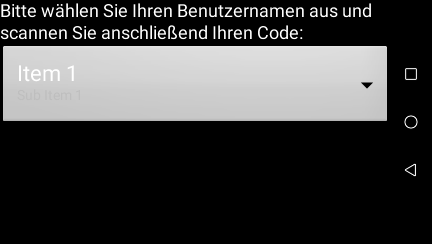
\includegraphics[scale=0.7]{Bilder/Abbildungen/login_mockup.png}}
	\caption{Login Mockup}
	\label{fig:sequenz_warenannnahme}
\end{figure}

Dies garantiert eine, entsprechend den eingeschränkten Möglichkeiten der Vuzix M100, zuverlässige und schnelle Anmeldung. Diese Anmeldemethode ist verständlicherweise nur für eine geringe Anzahl an Benutzern (ca. 30) effizient, jedoch wird davon ausgegangen, dass in einem Supermarkt in der Regel nicht mehr als 20 bis 30 Angestellte mit der Warenannahme/-einräumung beauftragt werden.\\
Die Anzeige aller möglichen Nutzernamen könnte ein Sicherheitsrisiko darstellen. Der Benutzername ist -- im Gegensatz zum Passwort -- zumindest gegenüber den anderen Mitarbeitern, die Zugriff auf die Brille haben, kein Geheimnis und kann bekannt sein.\\

Auch bei der Passworteingabe gibt es ähnliche Probleme, jedoch muss hier darauf geachtet werden, dass Passwörter ausschließlich dem jeweiligen Benutzer (und eventuell dem Systemadministrator) bekannt sein dürfen \bzw nur im Besitz des Benutzers liegen dürfen. Eine Auswahl aus einer Liste und die Eingabe per Spracherkennung sind somit nicht nur aus Sicht der Bedienung, sondern vor allem aus Sicherheitsgründen nicht praktikabel.\\
Ein Passwort, das auf Gesten basiert, ist aufgrund der geringen Anzahl an Variationen und möglichen Kombinationen ebenfalls nicht sicher. Die Passworteingabe muss daher über die vierte Eingabemöglichkeit getätigt werden: die Eingabe über Barcodes/QR-Codes mit Hilfe der Kamera.\\

Sobald der Benutzer seinen Benutzernamen aus der Liste ausgewählt hat, wird die Kamera, sowie eine Bibliothek zur Erkennung von QR-Codes gestartet. Der Benutzer scannt seinen persönlichen QR-Code, der in einen String mit einer Länge von 64 Zeichen umgewandelt wird. Diese Daten werden an den Server weitergeleitet, der die Anmeldung schließlich bestätigt (bei korrekter Kombination) oder widerruft (bei ungültigen Login-Daten). Bei korrekter Authentifizierung gibt der Server einen \acl{JWT} zurück, welcher bei allen weiteren Anfragen an den Server mitgeschickt werden muss und auf dort auf Korrektheit überprüft wird. Bei einem ungültigen Login erhält die App ausschließlich eine Fehlermeldung, weitere Anfragen werden aufgrund des fehlenden \acs{JWT} nicht ausgeführt.\\

Der QR-Code kann mit Hilfe der Weboberfläche generiert werden, oder es kann ein bestehender Code aktiviert werden (siehe Kapitel \ref{cha:impl_web} (\nameref{cha:impl_web})). Der QR-Code kann durch den Benutzer aufbewahrt werden; sollte der Code in unbefugte Hände gelangen, kann ein neuer Code generiert werden. Außerdem ist es möglich, vorhandene Codes zu verwenden, wie \zB ein Code auf der persönlichen Firmen-Zugangskarte des Benutzers\\
Die benötigte Sicherheit und das effiziente Anmelden an die Anwendung ist mit dieser Lösung gewährleistet.

\subsubsection{\acs{AuthN} gegenüber dem Server}
\label{cha:authn_server}
Im letzten Kapitel wurde beschrieben, wie sichergestellt wird, dass sich nur bekannte und authorisierte Benutzer anmelden können. Dass dies nicht unbedingt ausreichend ist, verdeutlicht das folgende Szenario:
\begin{quote}
\textit{Ein Angestellter einer Filiale, der mit der Warenannahme beauftragt ist und somit für die Nutzung der Brille freigeschaltet ist, lässt seinen Firmenausweis beim Einräumen in einem öffentlichen Bereich liegen. Auf dem Firmenausweis sind sowohl der vollständige Name, als auch der QR-Code, der für die Authentifizierung genutzt wird, aufgedruckt. Ein Angreifer, der Zugriff auf das System bekommen möchte, entdeckt dies und fotografiert den Firmenausweis ab.}
\end{quote}
Im oben dargestellten Szenario sind die persönlichen Benutzerdaten -- ohne Wissen des Opfers -- gestohlen worden. Der Angreifer hat zwar keinen Zugriff auf eine im Markt vorhandene \ac{AR}-Brille, aber eventuell ist er im Besitz der App und hat diese auf einem eigenen Android-Gerät installiert. Ist das Firmennetzwerk zusätzlich noch schlecht abgesichert, \zB durch Nutzung des veralteten \ac{WEP} Verschlüsselungsprotokolls, so kann sich der Angreifer mit seinem eigenen Android-Gerät und über die Anmeldedaten des Angestellten auf dem Server authentifizieren. Er kann den Warenbestand nun entsprechend manipulieren und der Filiale Schaden zufügen.\\

Um dies zu verhindern, wurde eine Zwei-Faktor-Authentifizierung in die Anwendung integriert. Somit muss sich nicht nur der Benutzer, sondern auch die \ac{AR}-Brille \bzw das benutzte Gerät gegenüber dem Server authentifizieren.\\
Eine \ac{MAC}-Adresse und somit das dazugehörige Gerät werden durch einen Eintrag in der Datenbank registriert. Für jedes Gerät wird ein Name, sowie die \ac{MAC}-Adresse vergeben und ein Flag gesetzt, ob dieses Gerät aktuell aktiv sein soll. Das registrierte Gerät kann sich somit gegenüber dem Server erfolgreich identifizieren.\\

Die App liest dazu beim Starten der Anwendung die \ac{MAC}-Adresse des Gerätes aus und speichert diese in der für den Login zuständigen Klasse ab. Die \ac{MAC}-Adresse ist die Hardware-Adresse des Gerätes, hat einen gerätegebundenen, einzigartigen Charakter und ist so ein hinreichendes Identifizierungsmerkmal eines Gerätes.\\
Sobald sich der Benutzer anmeldet (also seinen Benutzernamen ausgewählt hat und den persönlichen QR-Code eingescannt hat), wird die \ac{MAC}-Adresse an die Login-Daten angehängt und eine Anfrage (durch Ausführen des \emph{Authentication}-Service der REST API\footnote{s. Kapitel \ref{cha:impl_api}\nameref{cha:impl_api}}) an den Server mit allen Daten (\ac{MAC}-Adresse, Benutzer, Passwort) geschickt. Ist die \ac{MAC}-Adresse gültig und im System freigegeben, liefert der Server den \ac{JWT}, ansonsten gibt es eine Fehlermeldung und alle weiteren Anfragen werden abgelehnt.

\subsection{\acf{AuthZ}}
Die \acl{AuthZ} prüft die Berechtigungen der bereits vorhandenen Identifikation. Bei der Benutzung der App gibt es sowohl für das Gerät, als auch für den Benutzer ausschließlich 2 Berechtigungsstufen:
\begin{itemize}
	\item Benutzer/Gerät hat die Berechtigung, Daten zu lesen/bearbeiten/löschen,
	\item Benutzer/Gerät hat keine Berechtigung, auf die Daten zuzugreifen.
\end{itemize}

Die \acl{AuthZ} findet daher zeitgleich zu der \acl{AuthN} statt. Der \ac{JWT} wird ausschließlich bei erfolgreicher Identifikation und Berechtigung zurückgegeben, ansonsten gibt es eine entsprechende Fehlermeldung.\\

Das Gerät autorisiert sich gegenüber dem Server über das Flag, welches bestimmt, ob das Gerät aktuell im System aktiv ist. Ist dieses Flag gesetzt, besitzt dieses Gerät (\zB \acs{AR}-Brille) volle Berechtigung zur Nutzung der \acs{API} und weitere Anfragen werden bei gültigem \ac{JWT} übergeben, ansonsten werden alle weiteren Anfragen abgelehnt. Diese \acl{AuthZ} macht Sinn, sollte das Gerät vorübergehend aus dem operativen Betrieb genommen werden. Das Gerät kann gesperrt und reaktiviert werden, ohne dass es aus dem System gelöscht und anschließend wieder registriert werden muss.\\

Da ein Benutzer ebenfalls nur diese zwei Berechtigungsstufen beim Benutzen der App besitzt, wird die Anfrage ähnlich der Brille ausgeführt. Ein Benutzer besitzt in seinem Datenbank-Eintrag in der Spalte \emph{role\_device}~ entweder eine 1 (true) und wird zur Nutzung der Brille autorisiert, oder eine 0 (false) und der Server meldet einen entsprechenden Fehler zurück.\\

Weitere Berechtigungsstufen werden an dieser Stelle nicht benötigt, da ein Angestellter, der mit der Warenannahme oder -einräumung beauftragt ist, die gesamte App-Funktionalität inklusive aller Schreibrechte benutzt, jedoch ein Angestellter, der keine der Aufgaben durchführt, von vornherein keinen Zugriff auf die Smartglass haben muss.
